\thispagestyle{normalpage}

\begin{center}
    \large \textbf{CHAPITRE II} \\[0.3em]
    \large \textbf{ANALYSE ET CONCEPTION : VERS UNE ARCHITECTURE DISTRIBUÉE}
\end{center}
\addcontentsline{toc}{chapter}{CHAPITRE II - ANALYSE ET CONCEPTION}
\label{page:chapitre2}

Ce chapitre expose la réflexion conceptuelle menée pour répondre aux exigences de scalabilité et de haute disponibilité de Techcare. Nous y abordons les fondements théoriques des systèmes distribués, le découpage métier via le Domain-Driven Design (DDD) et la modélisation des flux de données.

\section{II.1 Analyse de l'existant et État de l'Art}
\label{sec:analyse_art}

\begin{figure}[htbp]
    \centering
    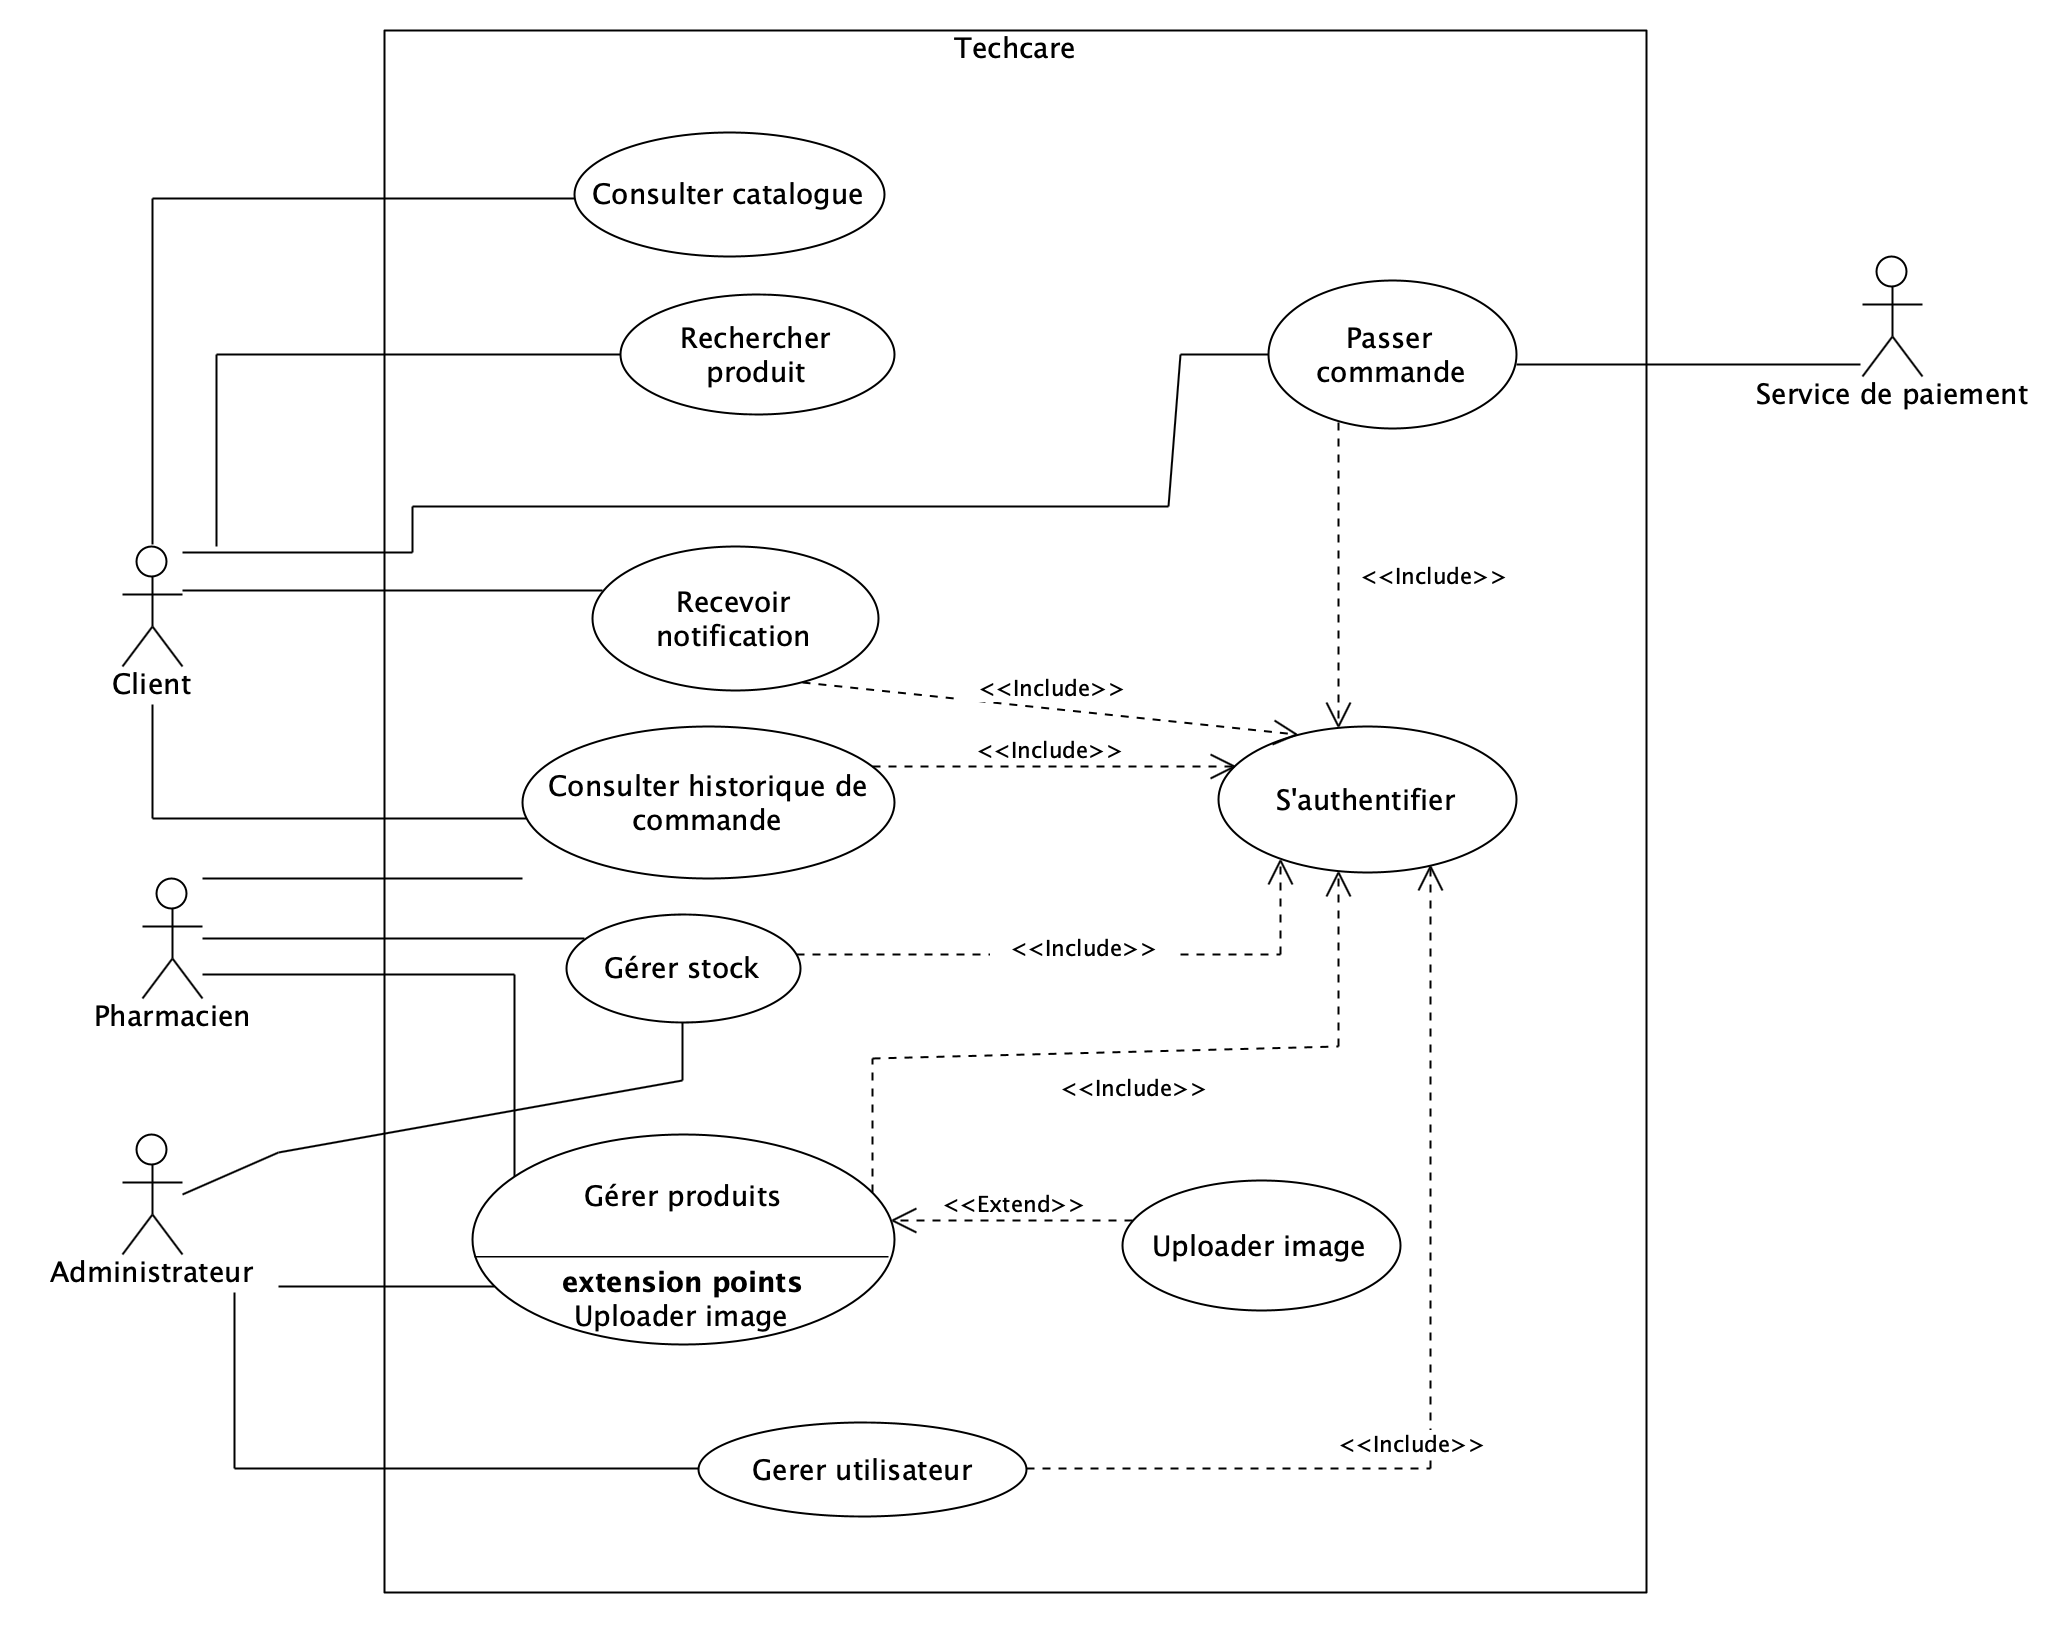
\includegraphics[width=\textwidth]{diagrams/use_case/use_case.png}
    \caption{Diagramme de cas d'utilisation du système Techcare}
    \vspace{0.2cm}\small\textit{Source : Auteur}
    \label{fig:use_case}
\end{figure}

L'analyse de ce diagramme de cas d'utilisation permet de dégager les points suivants :
\begin{itemize}
    \item \textbf{Interactions et Acteurs} : Ce diagramme illustre les interactions fondamentales entre les trois acteurs principaux (Client, Pharmacien et Administrateur) et les fonctionnalités clés, couvrant l'intégralité du cycle de vie médical, de la recherche à la délivrance.
    \item \textbf{Périmètre et Dépendances} : Il met en évidence les relations de dépendance, notamment l'authentification systématique requise pour les actions sensibles, et sert de base pour définir le périmètre fonctionnel du système Techcare.
\end{itemize}


\subsection{II.1.1 Évolution des architectures logicielles : Un parcours historique}
L'histoire de l'ingénierie logicielle est marquée par une oscillation constante entre centralisation et décentralisation, motivée par la recherche d'un équilibre entre contrôle, performance et agilité.

\begin{enumerate}
    \item \textbf{L'ère des Mainframes (années 1960-1980)} : Le calcul était totalement centralisé sur des machines massives. Les utilisateurs interagissaient via des "terminaux passifs" sans puissance de calcul propre. Bien que robuste, ce modèle offrait une flexibilité nulle et un coût d'entrée prohibitif.
    
    \item \textbf{L'ère Client-Serveur (années 1990)} : Avec l'avènement du PC, l'intelligence a été répartie. Le modèle \textit{2-tier} (une application lourde communiquant avec une base de données) a permis l'essor des interfaces graphiques complexes, mais posait des problèmes majeurs de maintenance (chaque mise à jour nécessitait une réinstallation sur chaque poste client).
    
    \item \textbf{L'Architecture N-tier et le Monolithe Web (années 2000)} : Pour résoudre les problèmes du client-serveur, le calcul est revenu vers le centre (serveur d'application), mais de manière structurée en couches (Présentation, Métier, Données). C'est l'âge d'or des architectures monolithiques bien structurées, où l'intégralité de la logique réside dans un unique bloc déployable.
    
    \item \textbf{SOA (Service-Oriented Architecture)} : Avant les microservices, la SOA a tenté de modulariser l'entreprise. En utilisant des protocoles lourds (SOAP, XML) et un bus de communication central (ESB), elle visait la réutilisabilité. Cependant, la complexité de l'ESB créait souvent un nouveau goulot d'étranglement centralisé.
    
    \item \textbf{La révolution des Microservices et du Cloud (2010-Aujourd'hui)} : En réponse aux besoins de "Scale" des géants du web (Netflix, Amazon), le concept de microservices a émergé. Il prône un découplage total, où chaque service est une unité autonome.
\end{enumerate}

Le passage du monolithe aux microservices chez Techcare n'est donc pas une simple tendance, mais l'aboutissement de cette évolution vers la décentralisation contrôlée, répondant à la **loi de Conway** : pour que Techcare soit agile, son architecture doit refléter une structure de communication fluide et distribuée.


\subsection{II.1.2 L'Architecture Monolithique : Analyse du Modèle Traditionnel}
L'architecture monolithique constitue le modèle canonique de conception logicielle. Bien qu'aujourd'hui souvent critiquée face à l'essor des microservices, elle a dominé l'industrie pendant des décennies et reste pertinente pour nombre de projets. Pour Techcare, comprendre ses mécanismes est crucial pour justifier la transition.

\subsubsection{II.1.2.1 Caractéristiques et Modèle de Déploiement}
Dans un système monolithique, l'intégralité de la logique métier, de l'accès aux données et de l'interface est compilée dans un unique artefact exécutable. Cette structure implique plusieurs contraintes techniques :
\begin{itemize}
    \item \textbf{Couplage Spatial et Temporel} : Tous les composants s'exécutent dans le même espace mémoire et partagent le même cycle de vie. Un redémarrage du serveur pour mettre à jour le module de facturation rend momentanément indisponible le catalogue de médicaments.
    \item \textbf{Gestion des Ressources Partagées} : Le moteur d'exécution (JVM, Node.js, etc.) gère un pool de threads unique. Une boucle infinie ou une fuite de mémoire dans un composant "non critique" peut saturer les ressources et provoquer l'arrêt total du système.
    \item \textbf{Base de données Centralisée} : Le monolithe communique généralement avec un unique schéma relationnel (Shared Database), facilitant les jointures complexes mais créant un point de contention majeur lors de la montée en charge.
\end{itemize}

\subsubsection{II.1.2.2 Atouts Techniques et Opérationnels}
Avant d'atteindre ses limites, le monolithe offre des avantages indéniables :
\begin{itemize}
    \item \textbf{Intégrité Transactionnelle (ACID)} : Les opérations inter-modules bénéficient de transactions locales garanties par le moteur de base de données, évitant la complexité des transactions distribuées (Saga).
    \item \textbf{Latence Zéro Inter-Composants} : Les échanges d'informations se font par passage de références en mémoire. Contrairement aux microservices, il n'y a ni sérialisation (JSON/Protobuf), ni latence réseau, ni risque de timeout entre les fonctions.
    \item \textbf{Facilité de Refactoring} : Grâce au typage fort et à la vision globale du code, les outils de l'IDE permettent de renommer ou de restructurer des composants à travers toute l'application en une seule opération sécurisée.
\end{itemize}

\subsubsection{II.1.2.3 Limites Structurelles et le phénomène "Big Ball of Mud"}
Pour Techcare, le monolithe a fini par dériver vers ce que Brian Foote et Joseph Yoder appellent une **"Big Ball of Mud"** (grosse boule de boue) : une architecture sans structure apparente où le couplage devient si dense que toute modification devient imprévisible.
\begin{itemize}
    \item \textbf{Lourdeur du Continuous Deployment (CD) et complexité du débogage} : Le temps de build n'est pas vraiment le problème majeur, le débogage oui. Avec la complexité croissante du code monolithique, identifier la source d'une régression lors d'un déploiement nécessitait de parcourir une base de code dense et fortement couplée, allongeant considérablement le temps de résolution des incidents.
    \item \textbf{Scalabilité Inefficace} : La scalabilité est obligatoirement "homogène". Pour absorber un pic de trafic sur la recherche de médicaments, nous devions dupliquer l'intégralité du socle (incluant les modules lourds et inutilisés en lecture seule), entraînant un surcoût d'infrastructure inutile.
    \item \textbf{Obsolescence Technologique Subie} : Le système est "prisonnier" de ses choix initiaux. Passer d'une version majeure de framework ou changer de langage est une mission quasi-impossible car elle impacterait des millions de lignes de code interdépendantes.
\end{itemize}

\textbf{Bilan comparatif :}
Pour synthétiser cette transition architecturale, le tableau \ref{tab:monolith_vs_microservices} met en évidence les différences fondamentales justifiant le passage aux microservices pour la plateforme Techcare.

\begin{table}[htbp]
    \centering
    \renewcommand{\arraystretch}{1.3}
    \begin{tabular}{|p{3.5cm}|p{5cm}|p{5cm}|}
        \hline
        \textbf{Critère} & \textbf{Ancien Monolithe} & \textbf{Nouvelle Architecture (Microservices)} \\
        \hline
        \textbf{Déploiement} & Lourd et risqué. Un seul artefact englobant tout. & Agile et indépendant par service (conteneurs isolés). \\
        \hline
        \textbf{Scalabilité} & Homogène. Duplication totale de l'application (lourdeur matérielle). & Ciblée. Seuls les services sollicités sont dupliqués. \\
        \hline
        \textbf{Tolérance aux pannes} & Point de défaillance unique (SPOF). Tout le système tombe en cas de crash. & Haute résilience. L'échec d'un service n'impacte pas le reste. \\
        \hline
        \textbf{Persistance} & Base de données unique et centralisée (couplage fort). & Base de données par service (Persistance Polyglotte). \\
        \hline
        \textbf{Stack technologique} & Unique et figé (Risque d'obsolescence). & Hétérogène (Le bon outil pour la bonne tâche). \\
        \hline
    \end{tabular}
    \caption{Comparaison entre l'architecture monolithique et microservices}
    \vspace{0.2cm}\small\textit{Source : Auteur}
    \label{tab:monolith_vs_microservices}
\end{table}

\subsection{II.1.3 Le framework NestJS : Historique et Structure}
Face aux limites de l'architecture monolithique, la mise en œuvre de microservices modernes requiert des outils robustes. C'est dans ce contexte que s'inscrit NestJS.

\subsubsection{Historique et genèse}
Créé en 2017 par Kamil Myśliwiec, NestJS (souvent appelé simplement Nest) est un framework pour la création d'applications Node.js côté serveur. Historiquement, l'écosystème Node.js était dominé par des bibliothèques minimalistes comme Express.js ou Koa. Bien que ces outils offrent une grande flexibilité, ils n'imposent aucune structure architecturale. Cela conduit fréquemment à du code non structuré (spaghetti code) dans les projets d'envergure. NestJS a été conçu pour résoudre ce problème architectural en s'inspirant fortement des concepts d'Angular.

\subsubsection{Concepts fondamentaux et architecture de NestJS}
NestJS utilise nativement TypeScript (bien qu'il supporte JavaScript pur) et combine des éléments de Programmation Orientée Objet (POO), de Programmation Fonctionnelle (FP) et de Programmation Réactive Fonctionnelle (FRP). 


L'architecture de NestJS s'articule autour de plusieurs notions clés qu'il est indispensable de maîtriser :

\begin{itemize}
    \item \textbf{Le CLI (Command Line Interface)} : L'outil \texttt{NestCLI} est essentiel pour l'initialisation et le développement. Il permet de générer rapidement des projets, de scaffolder des éléments (modules, contrôleurs, services) tout en respectant scrupuleusement les conventions de nommage et de structure du framework.
    
    \item \textbf{Modules} : Un module est une classe annotée avec le décorateur \texttt{@Module()}. Il permet d'encapsuler logiquement un domaine métier (par exemple, un \texttt{UsersModule} ou \texttt{ProductsModule}) en regroupant ses contrôleurs et ses providers. Chaque application possède un module racine. Cette approche encourage fortement la séparation des préoccupations, idéale pour concevoir des microservices indépendants.
    \begin{figure}[htbp]
    \centering
    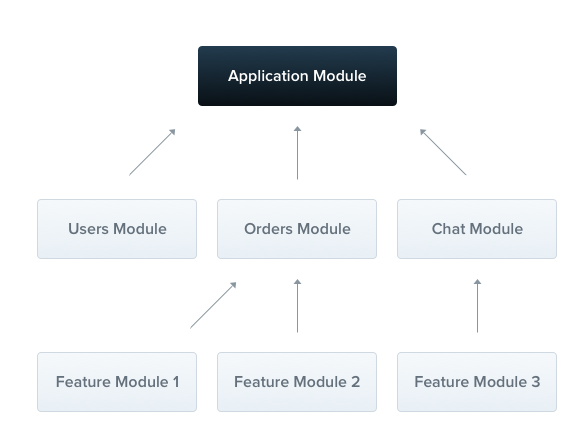
\includegraphics[width=0.8\textwidth]{diagrams/modules_nestjs.png}
    \caption{Architecture du module NestJS}
    \vspace{0.2cm}\small\textit{Source : nestjs.com}
    \label{fig:modules_nestjs}
\end{figure}
    \item \textbf{Contrôleurs (Controllers)} : Annotés par \texttt{@Controller()}, ils constituent la couche de présentation. Leur unique responsabilité est de réceptionner les requêtes entrantes, d'extraire les paramètres (via des décorateurs comme \texttt{@Body()}, \texttt{@Param()}) et de déléguer la logique métier aux services. Dans un contexte microservices, ils gèrent aussi le trafic asynchrone (RabbitMQ, TCP) via \texttt{@MessagePattern}.
    
    \item \textbf{Services et Providers} : Les services sont les porteurs de la logique métier (Business Logic) et de l'accès aux bases de données. Dans NestJS, presque toute classe utilitaire (services, repositories, factories) est considérée comme un "Provider" (annotée via \texttt{@Injectable()}).
    
    \item \textbf{L'Injection de Dépendances (Dependency Injection - DI)} : C'est le cœur du système NestJS. Au lieu d'instancier manuellement une classe (via le mot-clé \texttt{new}), NestJS gère un conteneur IoC (Inversion of Control) qui injecte automatiquement les instances nécessaires (les Providers) dans les classes qui en ont besoin (comme les Contrôleurs). Cela garantit un code lâchement couplé, hautement modulaire et facilement testable.
\end{itemize}

Grâce à cette structure rigoureuse et standardisée, NestJS s'impose comme une référence incontournable pour la construction d'architectures distribuées complexes.

\subsubsection{Avantages, inconvénients et performances de NestJS}

L'adoption de NestJS pour Techcare repose sur un compromis technique équilibré. Il convient d'en évaluer les bénéfices et les limites.

\textbf{Les Avantages majeurs :}
\begin{itemize}
    \item \textbf{Maintenabilité et scalabilité d'équipe} : L'architecture fortement opinionnée oblige tous les développeurs à suivre la même structure, ce qui simplifie l'intégration de nouveaux membres et la revue de code.
    \item \textbf{Testabilité} : L'injection de dépendances (DI) permet de créer facilement des \textit{Mocks} et des \textit{Stubs} pour isoler les composants lors des tests unitaires.
    \item \textbf{Agnosticisme du protocole} : NestJS s'adapte naturellement aux microservices en masquant la complexité des protocoles (HTTP, WebSockets, RabbitMQ, gRPC) derrière une API uniforme.
\end{itemize}

\textbf{Les Inconvénients :}
\begin{itemize}
    \item \textbf{Courbe d'apprentissage abrupte} : Contrairement à Express.js qui s'apprend en quelques heures, NestJS nécessite une maîtrise de TypeScript, des décorateurs, de l'Inversion de Contrôle (IoC) et de RxJS.
    \item \textbf{Surcharge (Overhead) initiale} : Le framework embarque beaucoup de bibliothèques par défaut, générant une empreinte mémoire légèrement supérieure et un temps de démarrage plus long (Cold Start), ce qui peut être un frein dans des architectures Serverless (FaaS).
\end{itemize}

\textbf{Analyse des performances (Benchmark) :}
En termes de performances brutes, NestJS ajoute une légère couche d'abstraction (overhead) s'il s'exécute sur le moteur par défaut (Express.js). Un benchmark classique de requêtes simples ("Hello World") montre que :
\begin{itemize}
    \item \textbf{Express.js (natif)} : \(\sim\) 15 000 requêtes par seconde.
    \item \textbf{NestJS (sous Express)} : \(\sim\) 12 000 requêtes par seconde (en raison de l'interception et de l'injection de dépendances).
\end{itemize}
Toutefois, NestJS pallie cet écart en permettant de basculer son moteur sous-jacent sur \textbf{Fastify}. Lorsqu'il est configuré avec Fastify, NestJS atteint jusqu'à \textbf{30 000 requêtes par seconde}, dépassant largement Express.js tout en conservant son architecture robuste. Pour Techcare, cette modularité garantit que l'architecture logicielle ne deviendra pas un goulot d'étranglement lors de la montée en charge.

\section{II.2 Fondements Théoriques et Contraintes Distribuées}
\label{sec:theorie}

\subsection{II.2.1 Le Théorème CAP : Le dilemme de la distribution}
Formulé par Eric Brewer, le théorème CAP stipule que pour un système informatique distribué, il est impossible de garantir simultanément plus de deux des trois propriétés suivantes :
\begin{itemize}
    \item \textbf{Consistance (Consistency)} : Tous les nœuds voient les mêmes données au même moment.
    \item \textbf{Disponibilité (Availability)} : Chaque requête reçoit une réponse (succès ou échec), sans garantie qu'elle contienne la version la plus récente.
    \item \textbf{Partition Tolerance} : Le système continue de fonctionner malgré la perte de messages ou la défaillance d'une partie du réseau.
\end{itemize}

Pour Techcare, notre choix s'est porté sur une architecture **AP (Availability and Partition Tolerance)**. Dans un contexte pharmaceutique, il est préférable qu'un client puisse consulter le catalogue de médicaments (quitte à voir un stock légèrement désynchronisé de quelques secondes) plutôt que de se confronter à une erreur 500 bloquante. Nous adoptons donc le modèle de \textbf{Consistance Éventuelle} (\textit{Eventual Consistency}), où les données se propagent de manière asynchrone via RabbitMQ.

\subsection{II.2.2 Patterns de Résilience : Prévenir l'effet domino}
L'architecture distribuée multiplie les points de défaillance réseau. Afin de prévenir la propagation des pannes (effet domino), notre phase de conception théorique intègre plusieurs patrons d'architecture (patterns) majeurs de l'état de l'art, dont l'implémentation effective en production constitue un axe d'amélioration clé pour la plateforme :
\begin{itemize}
    \item \textbf{Circuit Breaker (Disjoncteur)} : Ce pattern surveille les échecs d'un service distant. S'ils dépassent un seuil, le disjoncteur "s'ouvre" et redirige immédiatement les appels vers un mode dégradé (ex: cache ou message d'erreur rapide), évitant ainsi d'épuiser les ressources du client en attendant un timeout.
    \item \textbf{Retry Pattern} : Pour les erreurs transitoires (micro-coupures réseau), le système réessaye automatiquement la requête avec une stratégie d'\textit{Exponential Backoff} pour ne pas saturer le service cible.
    \item \textbf{Bulkhead} : Inspiré des compartiments étanches des navires, ce pattern isole les pools de threads par service. Une saturation du \textit{Payment Service} n'impactera pas les performances du \textit{Product Service}.
\end{itemize}

\section{II.3 Découpage Métier : Le Domain-Driven Design (DDD)}
\label{sec:ddd_advanced}

Le Domain-Driven Design est au cœur de notre stratégie de décomposition. Il permet de s'assurer que le code reflète fidèlement la complexité métier.
\begin{itemize}
    \item \textbf{Bounded Contexts (Contextes Délimités)} : C'est la pierre angulaire de notre architecture. Au lieu d'avoir un modèle "Produit" géant, nous avons fragmenté ce concept. Dans le \textit{Product Manager},
     le produit est défini par son marketing (images, description). Dans l'\textit{Inventory Manager}, il est défini par sa logistique (code-barres, emplacement, seuil d'alerte).
    \item \textbf{Ubiquitous Language (Langage Commun)} : Nous avons structuré le code pour refléter fidèlement les notions de gestion d'officine (ex: l'événement \texttt{stock\_unavailable} pour la rupture de stock, et les types précis de mouvements de stock \texttt{RESERVATION} et \texttt{RELEASE} dans l'inventaire) plutôt que de simples opérations génériques d'incrémentation.
    \item \textbf{Aggregate Roots} : Chaque microservice gère une entité racine (ex: l'Ordre dans le service Commande) qui garantit l'intégrité de ses composants internes.
\end{itemize}

\section{II.4 Modélisation des Microservices et Communications}
\label{sec:patterns}

\subsection{II.4.1 API Gateway et Backend-for-Frontend (BFF)}
L'API Gateway constitue le point d'entrée unique pour tous les clients du système Techcare. Elle agit comme une couche d'abstraction entre les clients (Web, Mobile) et la complexité interne des microservices.

\begin{itemize}
    \item \textbf{Façade et Routage intelligent} : La Gateway redirige les requêtes entrantes vers les microservices appropriés en fonction de l'URL, masquant ainsi la topologie réelle du réseau interne et les adresses spécifiques de chaque service.
    \item \textbf{Agrégation de requêtes} : Pour optimiser les performances, elle peut fusionner les réponses de plusieurs services en un seul appel (ex: réunir les informations marketing de \textit{ProductService} et les niveaux de stock de \textit{InventoryService}), réduisant ainsi le "bavardage" réseau (\textit{chatter}) et la latence côté client.
    \item \textbf{Gouvernance centralisée} : Elle assure des fonctions transverses (\textit{Cross-Cutting Concerns}) telles que la terminaison SSL, la gestion des CORS, le \textit{Rate Limiting} pour prévenir les abus, et la validation initiale des jetons JWT.
    \item \textbf{Pattern BFF (Backend-for-Frontend)} : Cette approche nous permet de fournir des réponses adaptées aux besoins spécifiques de chaque interface utilisateur. Un client mobile recevra une version allégée des données pour économiser la bande passante, tandis qu'un portail administrateur pourra obtenir des informations plus denses.
\end{itemize}


\subsection{II.4.2 Chorégraphie : La force de l'asynchronisme}
Pour la communication entre services, nous avons exclu l'orchestration centralisée (qui crée un couplage fort et un SPOF) au profit de la **Chorégraphie** via le broker de messages RabbitMQ :
\begin{itemize}
    \item \textbf{Découplage temporel} : Un service peut émettre un événement même si le destinataire est temporairement hors ligne. Le broker garantit la persistance des messages.
    \item \textbf{Scalabilité horizontale} : Plusieurs instances d'un service peuvent consommer la même file d'attente pour traiter les tâches en parallèle.
    \item \textbf{Réduction de la latence} : L'utilisateur reçoit une réponse immédiate ("Commande acceptée"), tandis que le traitement lourd (paiement, notification, mise à jour des stocks) s'effectue en arrière-plan.
\end{itemize}

\begin{figure}[H]
    \centering
    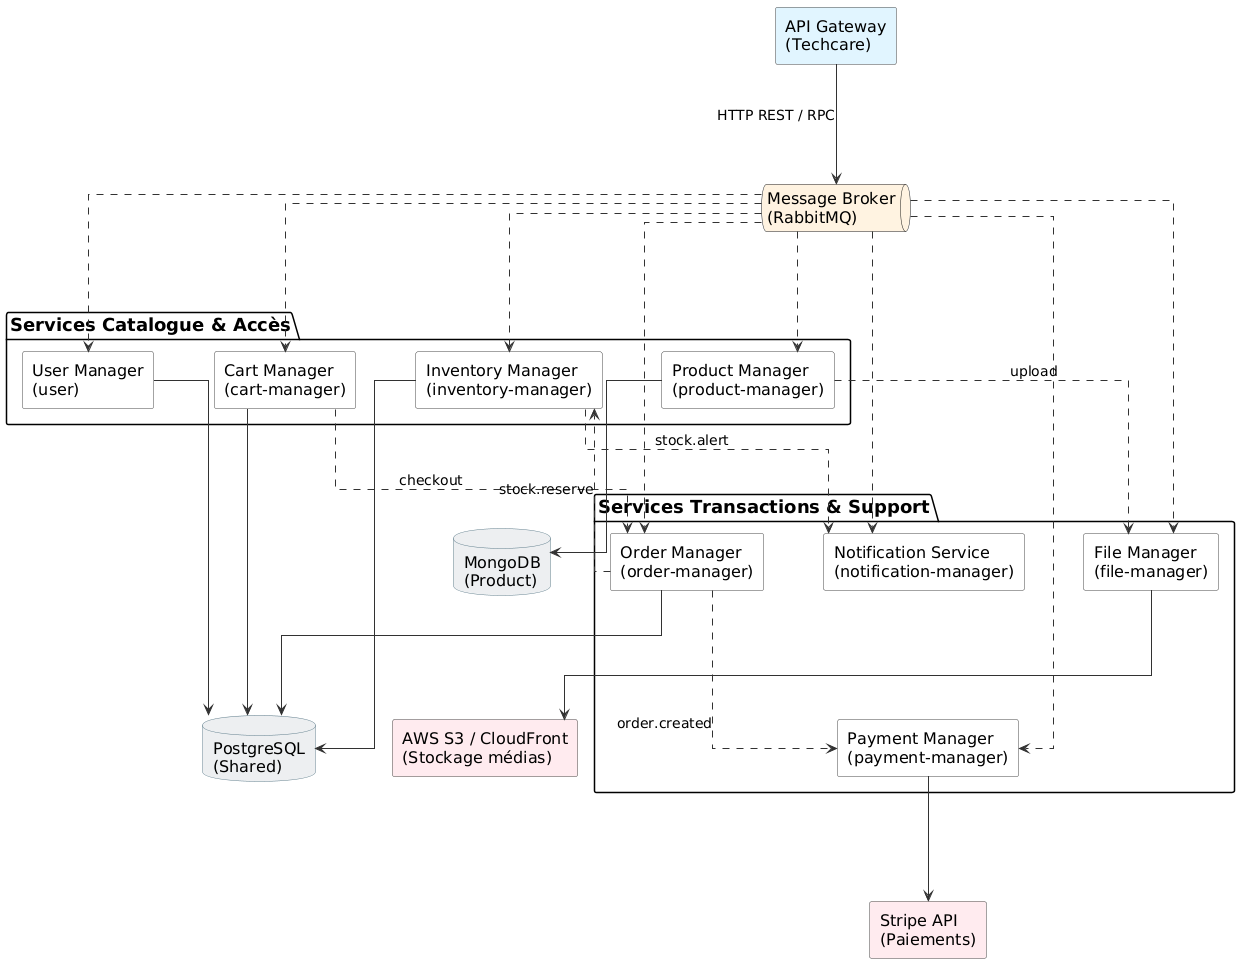
\includegraphics[width=\textwidth]{diagrams/class/interaction.png}
    \caption{Diagramme d'interaction et de communication des microservices (Chorégraphie)}
    \vspace{0.2cm}\small\textit{Source : Auteur}
    \label{fig:service_communication}
\end{figure}

L'analyse de ces flux d'interaction met en évidence le rôle central du Message Broker (RabbitMQ) dans la synchronisation des états et l'indépendance de la persistance (PostgreSQL et MongoDB).

\subsection{II.4.3 Modélisation des classes logiques des microservices}
Chaque microservice, bien qu'isolé dans son propre conteneur, adopte une architecture logicielle interne structurée et uniforme (Controller, Service, Entity). Le diagramme de classes global illustré par la figure \ref{fig:class_architecture} présente cette organisation structurelle. 
Pour des raisons de lisibilité et de clarté, les attributs et méthodes détaillés de chaque classe ne sont pas représentés afin de se concentrer sur l'architecture générale, l'organisation en packages et les relations entre composants logiques.


\begin{figure}[H]
    \centering
    \begin{tikzpicture}[
    scale=0.58,
    transform shape,
    node distance=1.0cm and 1.2cm,
    umlclass/.style={
        draw=black!70,
        fill=white,
        minimum width=3.3cm,
        minimum height=0.7cm,
        align=center,
        font=\small\sffamily\bfseries,
        rounded corners=2pt
    },
    note/.style={
        draw=orange!40,
        fill=orange!5,
        rounded corners=2pt,
        font=\scriptsize\sffamily,
        align=left,
        minimum width=2.6cm
    },
    frame/.style={
        draw=gray!30,
        fill=gray!3,
        rounded corners=4pt,
        inner sep=8pt
    },
    gateway_frame/.style={
        draw=blue!30,
        fill=blue!3,
        rounded corners=4pt,
        inner sep=8pt,
        minimum height=2cm
    }
]

    % ==========================================
    % NODES PLACEMENT
    % ==========================================

    % --- Package API Gateway (Top Center - y=10.0) ---
    \node[umlclass] (Gateway) at (0.0, 10.0) {Gateway};
    \node[umlclass] (JwtAuthGuard) at (4.0, 10.0) {JwtAuthGuard};

    % --- ROW 1 (TOP): Services (y = 6.0 to 2.0) ---
    
    % Col 1: User Manager Service
    \node[umlclass] (UserService) at (-9.0, 6.0) {UserService};
    \node[umlclass] (User) at (-9.0, 4.0) {User (Entity)};
    \node[umlclass] (Role) at (-9.0, 2.0) {«enum»\\Role};

    % Col 2: Product Manager Service
    \node[umlclass] (ProductController) at (-3.0, 6.0) {ProductController};
    \node[umlclass] (ProductService) at (-3.0, 4.0) {ProductService};
    \node[umlclass] (Product) at (-3.0, 2.0) {Product (Entity)};

    % Col 3: Inventory Manager Service
    \node[umlclass] (InventoryController) at (3.0, 6.0) {InventoryController};
    \node[umlclass] (InventoryService) at (3.0, 4.0) {InventoryService};
    \node[umlclass] (Inventory) at (3.0, 2.0) {Inventory (Entity)};

    % Col 4: Cart Manager Service
    \node[umlclass] (CartController) at (9.0, 6.0) {CartController};
    \node[umlclass] (CartService) at (9.0, 4.0) {CartService};
    \node[umlclass] (Cart) at (9.0, 2.0) {Cart (Entity)};

    % --- ROW 2 (BOTTOM): Services (y = -2.0 to -6.0) ---

    % Col 1: Order Manager Service
    \node[umlclass] (OrderController) at (-9.0, -2.0) {OrderController};
    \node[umlclass] (OrderService) at (-9.0, -4.0) {OrderService};
    \node[umlclass] (Order) at (-9.0, -6.0) {Order (Entity)};

    % Col 2: Payment Manager Service
    \node[umlclass] (PaymentController) at (-3.0, -2.0) {PaymentController};
    \node[umlclass] (PaymentService) at (-3.0, -4.0) {PaymentService};

    % Col 3: File Manager Service
    \node[umlclass] (FileController) at (3.0, -2.0) {FileController};
    \node[umlclass] (FileService) at (3.0, -4.0) {FileService};

    % Col 4: Notification Service
    \node[umlclass] (NotificationController) at (9.0, -2.0) {NotificationController};
    \node[umlclass] (NotificationService) at (9.0, -4.0) {NotificationService};


    % ==========================================
    % NOTES
    % ==========================================

    
    \node[note] (product_note) at (-3.0, 0.4) {
        \textbf{MongoDB}\\
        Schéma flexible pour\\
        spécifications produits
    };
    
    \node[note] (inventory_note) at (3.0, 0.4) {
        \textbf{PostgreSQL}\\
        Garanties ACID\\
        Gestion des stocks
    };
    
    \node[note] (order_note) at (-9.0, -7.6) {
        \textbf{PostgreSQL}\\
        Transaction Saga\\
        Gestion commandes
    };

    % ==========================================
    % BACKGROUND FRAMES (Packages)
    % ==========================================
    \begin{scope}[on background layer]
        % API Gateway Package
        \node[gateway_frame, fit=(Gateway) (JwtAuthGuard),
              label={[anchor=south west, font=\bfseries\small\sffamily, text=blue!70!black, xshift=6pt, yshift=2pt]north west:API Gateway}] (gateway_pkg) {};
              
        % ROW 1 (TOP):
        % User Manager Package
        \node[frame, fit=(UserService) (User) (Role),
              label={[anchor=south west, font=\bfseries\small\sffamily, text=gray!80!black, xshift=6pt, yshift=2pt]north west:User Manager Service}] (user_pkg) {};
              
        % Product Manager Package
        \node[frame, fit=(ProductController) (ProductService) (Product) (product_note),
              label={[anchor=south west, font=\bfseries\small\sffamily, text=gray!80!black, xshift=6pt, yshift=2pt]north west:Product Manager Service}] (product_pkg) {};
              
        % Inventory Manager Package
        \node[frame, fit=(InventoryController) (InventoryService) (Inventory) (inventory_note),
              label={[anchor=south west, font=\bfseries\small\sffamily, text=gray!80!black, xshift=6pt, yshift=2pt]north west:Inventory Manager Service}] (inventory_pkg) {};

        % Cart Manager Package
        \node[frame, fit=(CartController) (CartService) (Cart),
              label={[anchor=south west, font=\bfseries\small\sffamily, text=gray!80!black, xshift=6pt, yshift=2pt]north west:Cart Manager Service}] (cart_pkg) {};
              
        % ROW 2 (BOTTOM):
        % Order Manager Package
        \node[frame, fit=(OrderController) (OrderService) (Order) (order_note),
              label={[anchor=south west, font=\bfseries\small\sffamily, text=gray!80!black, xshift=6pt, yshift=2pt]north west:Order Manager Service}] (order_pkg) {};

        % Payment Manager Package
        \node[frame, fit=(PaymentController) (PaymentService),
              label={[anchor=south west, font=\bfseries\small\sffamily, text=gray!80!black, xshift=6pt, yshift=2pt]north west:Payment Manager Service}] (payment_pkg) {};
              
        % File Manager Package
        \node[frame, fit=(FileController) (FileService),
              label={[anchor=south west, font=\bfseries\small\sffamily, text=gray!80!black, xshift=6pt, yshift=2pt]north west:File Manager Service}] (file_pkg) {};
              
        % Notification Package
        \node[frame, fit=(NotificationController) (NotificationService),
              label={[anchor=south west, font=\bfseries\small\sffamily, text=gray!80!black, xshift=6pt, yshift=2pt]north west:Notification Service}] (notification_pkg) {};
    \end{scope}

    % ==========================================
    % CONNECTIONS (Pure Class Relations)
    % ==========================================

    % Gateway ..> JwtAuthGuard
    \draw[dashed, ->, >=stealth, thick] (Gateway) -- (JwtAuthGuard);
    
    % Internal layers (vertical Controller -> Service -> Entity)
    \draw[->, >=stealth, thick] (UserService) -- (User);
    \draw[->, >=stealth, thick] (User) -- (Role);

    \draw[->, >=stealth, thick] (ProductController) -- (ProductService);
    \draw[->, >=stealth, thick] (ProductService) -- (Product);
    
    \draw[->, >=stealth, thick] (InventoryController) -- (InventoryService);
    \draw[->, >=stealth, thick] (InventoryService) -- (Inventory);

    \draw[->, >=stealth, thick] (CartController) -- (CartService);
    \draw[->, >=stealth, thick] (CartService) -- (Cart);

    \draw[->, >=stealth, thick] (OrderController) -- (OrderService);
    \draw[->, >=stealth, thick] (OrderService) -- (Order);
    
    \draw[->, >=stealth, thick] (PaymentController) -- (PaymentService);
    \draw[->, >=stealth, thick] (FileController) -- (FileService);
    \draw[->, >=stealth, thick] (NotificationController) -- (NotificationService);

\end{tikzpicture}

    \caption{Diagramme de classes global de l'architecture microservices}
    \vspace{0.2cm}\small\textit{Source : Auteur}
    \label{fig:class_architecture}
\end{figure}

L'analyse de cette architecture de classes révèle deux aspects fondamentaux de la conception :
\begin{itemize}
    \item \textbf{Organisation Domain-Driven (DDD)} : Contrairement au monolithe, les entités sont regroupées par contextes délimités (Catalog, Inventory, Order), garantissant un faible couplage et permettant à chaque domaine de posséder sa propre logique métier indépendante.
    \item \textbf{Flexibilité et Évolutivité} : La structure met en évidence le rôle de l'API Gateway et la séparation des services, ce qui permet au système d'évoluer organiquement et de faciliter l'adoption de nouvelles technologies par service sans impacter l'ensemble du système.
\end{itemize}


\section{II.5 Architecture de Persistance et Base de Données}
\label{sec:persistance}

Le choix de la \textbf{Persistance Polyglotte} répond au besoin de performance :
\begin{itemize}
    \item \textbf{PostgreSQL (ACID)} : Indispensable pour l'Inventory Manager afin d'éviter le "Double Spending" de médicaments.
    \item \textbf{MongoDB (BASE)} : Idéal pour le Product Manager afin de stocker des métadonnées hétérogènes (composition, posologie, photos).
\end{itemize}


\subsection{II.5.1 Justification des choix technologiques}

Le tableau suivant synthétise les critères de sélection des bases de données :

\begin{table}[htbp]
    \centering
    \begin{tabular}{|p{4cm}|p{5cm}|p{5cm}|}
        \hline
        \textbf{Critère} & \textbf{PostgreSQL} & \textbf{MongoDB} \\
        \hline
        Modèle de données & Relationnel (schéma fixe) & Documentaire (schéma flexible) \\
        \hline
        Consistance & ACID stricte & Consistance éventuelle \\
        \hline
        Cas d'usage Techcare & Stocks, Utilisateurs & Catalogue produits \\
        \hline
        Performance & Excellent pour transactions & Excellent pour lectures massives \\
        \hline
    \end{tabular}
    \caption{Comparaison des systèmes de persistance retenus}
    \vspace{0.2cm}\small\textit{Source : Auteur}
    \label{tab:db_comparison}
\end{table}

\subsubsection{II.5.1.1 Justification du choix de PostgreSQL}

PostgreSQL a été retenu pour les services nécessitant une \textbf{intégrité transactionnelle stricte}. Voici les raisons détaillées de ce choix :

\begin{enumerate}[label=\alph*)]
    \item \textbf{Garanties ACID indispensables} : Pour le service \textbf{Inventory Manager}, la gestion des stocks de médicaments ne tolère aucune incohérence. Les propriétés ACID de PostgreSQL garantissent :
    \begin{itemize}
        \item \textbf{Atomicité} : Une opération de décrémentation de stock est soit totalement effectuée, soit totalement annulée.
        \item \textbf{Consistance} : Les contraintes de vérification (ex: \texttt{quantity >= 0}) sont appliquées.
        \item \textbf{Isolation} : Les verrous empêchent les réservations doubles simultanées.
        \item \textbf{Durabilité} : Les modifications sont persistées même en cas de panne.
    \end{itemize}

    \item \textbf{Support des contraintes relationnelles} : Le service \textbf{User Manager} exploite les relations entre tables. PostgreSQL impose l'intégrité référentielle, évitant les incohérences de données orphelines.

    \item \textbf{Performance des jointures complexes} : Les requêtes agrégées (ex: historique de commandes détaillé) bénéficient de l'optimiseur de PostgreSQL, très performant pour les jointures massives.

    \item \textbf{Typage strict et sécurité} : L'utilisation de Drizzle ORM avec PostgreSQL offre une sécurité type-safe dès la compilation, réduisant drastiquement les bugs.
\end{enumerate}

\subsubsection{II.5.1.2 Justification du choix de MongoDB}

MongoDB a été sélectionné pour le service \textbf{Product Manager} en raison de la nature hétérogène des produits pharmaceutiques.

\begin{enumerate}[label=\alph*)]
    \item \textbf{Flexibilité du schéma documentaire} : Les produits médicaux ont des caractéristiques variables (sirops, comprimés, dispositifs médicaux). MongoDB permet de stocker ces variations dans une même collection sans migration de schéma complexe.

    \item \textbf{Performance des lectures à grande échelle} : Le catalogue étant majoritairement consulté en lecture, MongoDB excelle grâce à son indexation avancée et son cache mémoire intégré.

    \item \textbf{Support natif des données imbriquées} : Un produit contient des tableaux d'images ou de contre-indications. MongoDB stocke ces données nativement, évitant les jointures SQL coûteuses.

    \item \textbf{Évolutivité sans migration} : L'ajout de nouveaux types de produits ne nécessite aucune modification de la structure de la base de données existante.
\end{enumerate}

\textbf{Conclusion sur la persistance (Trade-offs) :}
Bien que la persistance polyglotte offre une flexibilité maximale, elle impose une complexité opérationnelle accrue. L'équipe de développement doit maîtriser deux langages de requêtage différents et la gestion des sauvegardes (\textit{backups}) devient plus hétérogène, nécessitant des stratégies distinctes pour le relationnel et le documentaire.

\subsubsection{II.5.1.3 Justification des technologies applicatives et services tiers}

Le choix des outils de développement et des services externes a été guidé par des impératifs d'architecture distribuée et de sécurité de l'information.

\begin{enumerate}[label=\alph*)]
    \item \textbf{Le framework NestJS} : Comme détaillé précédemment dans l'état de l'art (Section II.1.3), NestJS s'est imposé naturellement pour structurer l'ensemble de nos microservices grâce à son architecture fortement modulaire, son typage strict (TypeScript) et son intégration native des flux asynchrones.

    \item \textbf{Stockage Objet (AWS S3) pour l'approche Stateless} : Dans une architecture distribuée, les conteneurs doivent être éphémères et sans état (\textit{stateless}). Si un microservice sauvegarde une image de produit localement sur son disque, cette donnée sera perdue au redémarrage du conteneur ou sera inaccessible pour les autres instances en cas de montée en charge (\textit{Scale-out}). L'utilisation d'un stockage objet déporté comme Amazon S3 permet de centraliser les médias de manière hautement disponible, tout en déchargeant nos serveurs applicatifs.

    \item \textbf{Délégation de paiement (Stripe) et conformité} : Le traitement des paiements en ligne soulève des contraintes légales et sécuritaires majeures, notamment la norme \textbf{PCI-DSS} (Payment Card Industry Data Security Standard). Traiter et stocker soi-même des données bancaires expose la plateforme à des risques de cyberattaques sévères. La délégation complète de cette logique à une passerelle spécialisée comme Stripe garantit une sécurité transactionnelle de niveau bancaire sans alourdir notre infrastructure.
\end{enumerate}

\textbf{Limites et contraintes identifiées :}
L'adoption de ces services infonuagiques (\textit{Cloud Computing}) n'est pas sans contreparties. La forte dépendance à des services tiers comme AWS S3 ou Stripe introduit un risque de \textbf{\textit{Vendor Lock-in}} (dépendance vis-à-vis d'un fournisseur unique). De plus, elle soumet le système à la disponibilité réseau de ces prestataires externes : si l'API de Stripe tombe en panne, le processus de commande sur Techcare est bloqué malgré la résilience de nos propres microservices.

\subsection{II.5.2 Gestion des transactions distribuées : Pattern Saga}

Dans une architecture microservices, l'absence de transaction globale (ACID) inter-services pose un défi majeur. Le pattern \textbf{Saga}, introduit par Hector Garcia-Molina et Kenneth Salem en 1987, apporte une solution élégante à ce problème.

\subsubsection{Définition formelle}
Une Saga est une séquence de transactions locales $T_1, T_2, ..., T_n$ où chaque transaction $T_i$ possède une transaction compensatoire $C_i$. Si une transaction $T_k$ échoue, le système exécute les compensations $C_{k-1}, C_{k-2}, ..., C_1$ dans l'ordre inverse pour annuler les effets des transactions déjà validées.

\textbf{Les deux approches de Saga :}

\subsubsection{II.5.2.1 Orchestration (Centralisée)}
Un coordinateur central (Orchestrator) pilote l'exécution des transactions.
\begin{itemize}
    \item \textbf{Avantages} : Visibilité complète du flux, facilité de debugging
    \item \textbf{Inconvénients} : Point de défaillance unique (SPOF)
\end{itemize}

\subsubsection{II.5.2.2 Chorégraphie (Décentralisée)}
\textit{Choix retenu pour Techcare.} Chaque service écoute des événements et déclenche ses propres actions.
\begin{itemize}
    \item \textbf{Avantages} : Pas de SPOF, meilleure scalabilité
    \item \textbf{Inconvénients} : Complexité accrue du monitoring
\end{itemize}

\subsubsection{Exemple concret : Commande de médicament}

Considérons le scénario où un client commande un médicament sur Techcare :

\textbf{Étapes de la Saga (Happy Path) :}
\begin{enumerate}
    \item \textbf{ProductService} : Vérifie la disponibilité du produit → Émet \texttt{ProductValidated}
    \item \textbf{InventoryService} : Réserve le stock → Émet \texttt{StockReserved}
    \item \textbf{PaymentService} : Traite le paiement → Émet \texttt{PaymentCompleted}
    \item \textbf{NotificationService} : Envoie confirmation → Émet \texttt{OrderConfirmed}
\end{enumerate}

\textbf{Scénario de compensation (Failure Path) :}
Si le \texttt{PaymentService} échoue à l'étape 3, les compensations suivantes sont déclenchées :
\begin{itemize}
    \item $C_2$ : \texttt{InventoryService} libère la réservation de stock
    \item $C_1$ : \texttt{ProductService} marque le produit comme disponible
    \item Notification d'échec envoyée au client
\end{itemize}

\textbf{Implémentation via RabbitMQ :}
Chaque service publie des événements dans des exchanges dédiés. Les autres services écoutent les événements qui les concernent via des queues. Cette architecture événementielle garantit la résilience : si un service est temporairement indisponible, les messages restent dans la queue jusqu'à son retour en ligne.

\begin{table}[htbp]
    \centering
    \begin{tabular}{|l|l|l|}
        \hline
        \textbf{Événement} & \textbf{Émetteur} & \textbf{Écouteur} \\
        \hline
        ProductValidated & ProductService & InventoryService \\
        \hline
        StockReserved & InventoryService & PaymentService \\
        \hline
        PaymentFailed & PaymentService & InventoryService \\
        \hline
        StockReleased & InventoryService & NotificationService \\
        \hline
    \end{tabular}
    \caption{Flux d'événements dans la Saga de commande}
    \vspace{0.2cm}\small\textit{Source : Auteur}
    \label{tab:saga_events}
\end{table}

Ce mécanisme de chorégraphie distribué est illustré techniquement par le diagramme de séquence présenté en section II.7.1 (page \pageref{fig:sequence_saga}).

\subsection{II.5.3 Traçabilité Distribuée : L'enjeu de l'observabilité}

Dans une architecture distribuée où une simple requête utilisateur peut traverser la Gateway et plusieurs microservices via RabbitMQ, la localisation de l'origine d'une panne devient extrêmement complexe. Si un "Timeout" survient, il est impossible de déterminer instantanément quel maillon de la chaîne a cédé en consultant les journaux standards.

Pour pallier cette perte de visibilité, notre conception intègre dès l'origine le concept de \textbf{Traçabilité Distribuée (Distributed Tracing)}. Ce pattern consiste à attacher un identifiant unique (Trace ID) à chaque requête entrante. Cet identifiant est ensuite propagé de service en service, permettant de reconstruire le cycle de vie complet de la transaction. L'implémentation de cette solution s'appuiera sur des standards ouverts afin d'offrir une vue globale (topologie réseau, temps de traitement de chaque nœud) et d'isoler rapidement les composants défaillants sans modifier la logique métier.

\section{II.6 Modélisation de la Sécurité : Zero Trust Architecture}
\label{sec:security_master}

Dans notre conception, nous n'accordons aucune confiance implicite au réseau interne.

\subsection{II.6.1 Architecture de sécurité en couches}
\begin{enumerate}
    \item \textbf{Authentification Stateless} : Utilisation de JWT signés par algorithme asymétrique (RS256).
    \item \textbf{Propagation d'identité} : Le jeton est transmis de service en service, permettant un audit complet de chaque action.
    \item \textbf{Chiffrement End-to-End et en transit} : 
    \begin{itemize}
        \item \textbf{Transactions financières} : Cryptage de bout en bout entre le client et Stripe (les données bancaires ne transitent jamais sur nos serveurs).
        \item \textbf{Données sensibles} : Utilisation de TLS 1.3 pour toutes les communications avec AWS S3 et entre l'API Gateway et les clients.
        \item \textbf{Sécurisation au repos} : Hachage des mots de passe via l'algorithme Bcrypt dans le User Service.
    \end{itemize}
\end{enumerate}

\begin{figure}[H]
    \centering
    \begin{tikzpicture}[
    node distance=1.0cm and 1.0cm,
    font=\footnotesize,
    >=Stealth,
    participant/.style={draw, fill=blue!10, draw=blue!40, rounded corners=3pt, minimum width=1.8cm, minimum height=0.7cm, align=center, font=\scriptsize\bfseries},
    actor/.style={draw, fill=teal!10, draw=teal!40, rounded corners=3pt, minimum width=1.8cm, minimum height=0.7cm, align=center, font=\scriptsize\bfseries},
    database/.style={draw, cylinder, shape border rotate=90, fill=orange!10, draw=orange!40, minimum width=1.6cm, minimum height=0.7cm, align=center, font=\scriptsize\bfseries}
]

    % --- PARTICIPANTS ---
    \node[actor] (User) at (0,0) {Utilisateur\\ (Client/Pharm)};
    \node[participant] (UI) at (2.5,0) {Frontend\\ (Nuxt)};
    \node[participant] (Gateway) at (5.5,0) {API\\ Gateway};
    \node[participant] (Auth) at (8.5,0) {User Manager\\ Service};
    \node[database] (DB) at (11.5,0) {PostgreSQL\\ (DB)};

    % --- LIFELINES ---
    \draw[dashed, gray!50] (User.south) -- (0,-12.0);
    \draw[dashed, gray!50] (UI.south) -- (2.5,-12.0);
    \draw[dashed, gray!50] (Gateway.south) -- (5.5,-12.0);
    \draw[dashed, gray!50] (Auth.south) -- (8.5,-12.0);
    \draw[dashed, gray!50] (DB.south) -- (11.5,-12.0);

    % --- ACTIVATIONS ---
    \draw[fill=teal!20, draw=teal!60] (2.42,-0.8) rectangle (2.58,-11.2);
    \draw[fill=violet!20, draw=violet!60] (5.42,-1.5) rectangle (5.58,-10.4);
    \draw[fill=olive!20, draw=olive!60] (8.42,-2.2) rectangle (8.58,-9.6);
    \draw[fill=orange!20, draw=orange!60] (11.42,-2.9) rectangle (11.58,-3.6);

    % --- MESSAGES ---
    
    % 1. User -> UI
    \draw[->, thick] (0,-0.8) -- node[above, font=\scriptsize] {Saisit Identifiants (Email, Password)} (2.42,-0.8);
    
    % 2. UI -> Gateway
    \draw[->, thick] (2.58,-1.5) -- node[above, font=\scriptsize] {POST /auth/login} (5.42,-1.5);
    
    % 3. Gateway -> Auth
    \draw[->, thick] (5.58,-2.2) -- node[above, font=\scriptsize] {login\_user(email, password)} (8.42,-2.2);
    
    % 4. Auth -> DB
    \draw[->, thick] (8.58,-2.9) -- node[above, font=\scriptsize] {Find user by email} (11.42,-2.9);
    
    % 5. DB --> Auth
    \draw[->, dashed, thick] (11.42,-3.6) -- node[above, font=\scriptsize] {User Record (Hashed Password)} (8.58,-3.6);
    
    % 6. Auth -> Auth (Bcrypt)
    \draw[->, thick] (8.58,-4.1) -- ++(0.5,0) -- node[midway, right, font=\scriptsize, align=left] {Comparer les\\ mots de passe (bcrypt)} ++(0,-0.4) -- (8.58,-4.5);

    % Box Alt : Identifiants valides / invalides
    \draw[draw=gray!40, fill=gray!2, fill opacity=0.3, rounded corners=2pt] (-0.3,-4.9) rectangle (12.0,-12.2);
    \node[anchor=north west, font=\scriptsize\bfseries\color{gray}] at (-0.3,-4.9) {alt : Identifiants valides};
    
    % 7. Auth -> Auth (Generate JWT)
    \draw[->, thick] (8.58,-5.3) -- ++(0.5,0) -- node[midway, right, font=\scriptsize, align=left] {Générer JWT\\ Access Token} ++(0,-0.4) -- (8.58,-5.7);
    
    % 8. Auth -> Gateway
    \draw[->, dashed, thick] (8.42,-6.4) -- node[above, font=\scriptsize] {Response: \{ user, accessToken \}} (5.58,-6.4);
    
    % 9. Gateway -> UI
    \draw[->, dashed, thick] (5.42,-7.0) -- node[above, font=\scriptsize] {200 OK + JWT} (2.58,-7.0);
    
    % 10. UI -> UI (Store JWT)
    \draw[->, thick] (2.58,-7.6) -- ++(0.5,0) -- node[midway, right, font=\scriptsize, align=left] {Stocker JWT dans\\ localStore/Vuex} ++(0,-0.4) -- (2.58,-8.0);
    
    % 11. UI -> User
    \draw[->, thick] (2.42,-8.5) -- node[above, font=\scriptsize] {Redirection vers Dashboard} (0,-8.5);
    
    % Else Line
    \draw[dashed, gray!40] (-0.3,-8.9) -- (12.0,-8.9);
    \node[anchor=north west, font=\scriptsize\bfseries\color{gray}] at (-0.3,-8.9) {else : Identifiants invalides};
    
    % 12. Auth -> Gateway
    \draw[->, dashed, thick] (8.42,-9.6) -- node[above, font=\scriptsize] {Error: Unauthorized} (5.58,-9.6);
    
    % 13. Gateway -> UI
    \draw[->, dashed, thick] (5.42,-10.4) -- node[above, font=\scriptsize] {401 Unauthorized} (2.58,-10.4);
    
    % 14. UI -> User
    \draw[->, thick] (2.42,-11.2) -- node[above, font=\scriptsize] {Message: Email ou mot de passe incorrect} (0,-11.2);

\end{tikzpicture}

    \caption{Diagramme de séquence de l'authentification utilisateur}
    \vspace{0.2cm}\small\textit{Source : Auteur}
    \label{fig:sequence_auth}
\end{figure}

Ce flux d'authentification met en exergue deux piliers de notre stratégie de sécurité :
\begin{itemize}
    \item \textbf{Authentification Stateless avec JWT} : Le diagramme détaille l'utilisation de jetons signés cryptographiquement (RS256) transmis au client, ce qui élimine le besoin de sessions persistantes sur le serveur et facilite la scalabilité horizontale.
    \item \textbf{Validation Décentralisée} : Cette approche délègue la vérification de l'identité à chaque microservice de manière autonome, supprimant les goulots d'étranglement centraux et renforçant la résilience globale lors de la navigation sur la plateforme.
\end{itemize}


\subsection{II.6.2 Gestion des rôles et permissions}

Le système implémente un contrôle d'accès basé sur les rôles (RBAC) :
\begin{itemize}
    \item \textbf{Admin} : Accès complet (CRUD produits, gestion stocks, utilisateurs)
    \item \textbf{Pharmacien} : Lecture catalogue, gestion commandes, mise à jour stocks
    \item \textbf{Client} : Consultation catalogue, passage de commandes
\end{itemize}

\section{II.7 Modélisation des Flux et Cas d'Usage}
\label{sec:use_cases}

Pour illustrer l'architecture, prenons le cas d'usage critique : "Passer une commande".

\subsection{II.7.1 Processus métier de commande}

Le flux se déroule ainsi :
\begin{enumerate}
    \item Le client envoie une requête HTTP POST à l'API Gateway
    \item La Gateway vérifie le JWT et route vers le Product Manager via RabbitMQ
    \item Le Product Manager valide la disponibilité
    \item Un événement "ProductReserved" est publié
    \item L'Inventory Manager écoute cet événement et décrémente le stock
    \item Une notification est envoyée au client via Socket.io
\end{enumerate}

\begin{figure}[H]
    \centering
    \begin{tikzpicture}[
    node distance=1.0cm and 1.0cm,
    font=\footnotesize,
    >=Stealth,
    startstop/.style={draw, rounded corners=10pt, fill=blue!10, draw=blue!50, minimum width=2.5cm, minimum height=0.6cm, align=center, thick},
    process/.style={draw, fill=gray!5, draw=gray!40, minimum width=3.0cm, minimum height=0.8cm, text width=2.8cm, align=center, rounded corners=3pt},
    decision/.style={draw, diamond, aspect=1.8, fill=orange!10, draw=orange!50, minimum width=2.5cm, minimum height=0.8cm, text width=2.1cm, align=center, inner sep=0pt},
    arrow/.style={->, thick}
]

    % --- GAUCHE : PROCESSUS CLIENT ---
    \node (start) [startstop] at (0,0) {Début};
    \node (consulte) [process] at (0,-1.5) {Client consulte\\ le catalogue};
    \node (recherche) [process] at (0,-3.0) {Recherche d'un\\ produit spécifique};
    \node (trouve) [decision] at (0,-4.75) {Produit trouvé ?};
    \node (trouve_non) [process] at (-4.0,-4.75) {Afficher "Produit\\ non trouvé"};
    \node (stop_left) [startstop] at (-4.0,-6.25) {Fin (Annulé)};
    
    \node (panier) [process] at (0,-6.5) {Ajouter au panier};
    \node (verif_panier) [process] at (0,-8.0) {Vérifier le contenu\\ du panier};
    \node (valider) [decision] at (0,-9.75) {Valider la\\ commande ?};
    \node (valider_non) [process] at (-4.0,-9.75) {Continuer les achats};
    
    \node (auth) [process] at (0,-11.5) {S'authentifier (JWT)};
    \node (adresse) [process] at (0,-13.0) {Saisir l'adresse\\ de livraison};
    \node (paiement_mode) [process] at (0,-14.5) {Sélectionner le\\ mode de paiement};

    % --- DROITE : TRAITEMENT SAGA ---
    \node (verif_dispo) [process] at (4.8,-1.5) {Vérification de la\\ disponibilité};
    \node (dispo_check) [decision] at (4.8,-3.0) {Stock disponible ?};
    \node (dispo_non) [process] at (8.8,-3.0) {Afficher rupture\\ de stock};
    \node (stop_right_dispo) [startstop] at (8.8,-4.75) {Fin (Annulé)};
    
    \node (reserve) [process] at (4.8,-4.75) {Réservation du stock};
    \node (pay_stripe) [process] at (4.8,-6.5) {Procéder au\\ paiement (Stripe)};
    \node (pay_check) [decision] at (4.8,-8.25) {Paiement réussi ?};
    
    \node (pay_non) [process] at (8.8,-8.25) {Libérer la réservation\\ de stock};
    \node (pay_err) [process] at (8.8,-9.75) {Afficher erreur\\ de paiement};
    \node (stop_right_pay) [startstop] at (8.8,-11.5) {Fin (Échec)};
    
    \node (confirm) [process] at (4.8,-10.0) {Confirmer la\\ commande};
    \node (notif) [process] at (4.8,-11.5) {Envoyer notification\\ de succès};
    \node (stop) [startstop] at (4.8,-13.0) {Fin (Succès)};

    % --- BOITE SAGA (BACKGROUND) ---
    \begin{scope}[on background layer]
        \node (saga_box) [draw=gray!40, dashed, fill=gray!3, rounded corners=8pt, inner sep=15pt,
            fit=(verif_dispo) (stop) (dispo_non) (pay_err) (stop_right_dispo) (stop_right_pay),
            label={[text=gray!70, font=\bfseries]above:Traitement Commande (Saga)}] {};
    \end{scope}

    % --- LIENS GAUCHE ---
    \draw [arrow] (start) -- (consulte);
    \draw [arrow] (consulte) -- (recherche);
    \draw [arrow] (recherche) -- (trouve);
    \draw [arrow] (trouve) -- node[left] {oui} (panier);
    \draw [arrow] (trouve) -- node[above] {non} (trouve_non);
    \draw [arrow] (trouve_non) -- (stop_left);
    \draw [arrow] (panier) -- (verif_panier);
    \draw [arrow] (verif_panier) -- (valider);
    \draw [arrow] (valider) -- node[left] {oui} (auth);
    \draw [arrow] (valider) -- node[above] {non} (valider_non);
    \draw [arrow] (auth) -- (adresse);
    \draw [arrow] (adresse) -- (paiement_mode);

    % --- BOUCLE CONTINUER ACHATS ---
    \draw [arrow] (valider_non.west) -- ++(-0.5,0) |- (consulte.west);

    % --- LIEN GAUCHE -> DROITE (SAGA) ---
    \draw [arrow] (paiement_mode.south) -- ++(0,-0.4) -- (2.4, -15.3) |- (verif_dispo.west);

    % --- LIENS DROITE ---
    \draw [arrow] (verif_dispo) -- (dispo_check);
    \draw [arrow] (dispo_check) -- node[left] {oui} (reserve);
    \draw [arrow] (dispo_check) -- node[above] {non} (dispo_non);
    \draw [arrow] (dispo_non) -- (stop_right_dispo);
    \draw [arrow] (reserve) -- (pay_stripe);
    \draw [arrow] (pay_stripe) -- (pay_check);
    \draw [arrow] (pay_check) -- node[left] {oui} (confirm);
    \draw [arrow] (pay_check) -- node[above] {non} (pay_non);
    \draw [arrow] (pay_non) -- (pay_err);
    \draw [arrow] (pay_err) -- (stop_right_pay);
    \draw [arrow] (confirm) -- (notif);
    \draw [arrow] (notif) -- (stop);

\end{tikzpicture}

    \caption{Diagramme d'activité du processus de commande}
    \vspace{0.2cm}\small\textit{Source : Auteur}
    \label{fig:activity_order}
\end{figure}

Ce processus métier peut être analysé selon deux axes principaux :
\begin{itemize}
    \item \textbf{Logique Métier et Décisions} : Ce flux retrace le cheminement critique d'une commande, soulignant les points de décision comme la validation des stocks ou le succès du paiement, et les bifurcations en cas d'erreur.
    \item \textbf{Optimisation de l'Expérience} : La visualisation de ces étapes a permis d'identifier les zones de contact utilisateur, facilitant l'intégration de notifications en temps réel pour informer le client de l'état d'avancement de son traitement.
\end{itemize}


\begin{figure}[H]
    \centering
    \begin{tikzpicture}[
    node distance=1.0cm and 1.0cm,
    font=\footnotesize,
    >=Stealth,
    participant/.style={draw, fill=blue!10, draw=blue!40, rounded corners=3pt, minimum width=1.6cm, minimum height=0.7cm, align=center, font=\scriptsize\bfseries},
    actor/.style={draw, fill=teal!10, draw=teal!40, rounded corners=3pt, minimum width=1.6cm, minimum height=0.7cm, align=center, font=\scriptsize\bfseries},
    queue/.style={draw, fill=orange!10, draw=orange!40, rounded corners=3pt, minimum width=1.6cm, minimum height=0.7cm, align=center, font=\scriptsize\bfseries}
]

    % --- PARTICIPANTS ---
    \node[actor] (Client) at (0,0) {Client};
    \node[participant] (Gateway) at (2.0,0) {API\\ Gateway};
    \node[participant] (Product) at (4.0,0) {Product\\ Service};
    \node[participant] (Inventory) at (6.0,0) {Inventory\\ Service};
    \node[participant] (Payment) at (8.0,0) {Payment\\ Service};
    \node[participant] (Notif) at (10.0,0) {Notification\\ Service};
    \node[queue] (MQ) at (12.2,0) {RabbitMQ\\ (Broker)};

    % --- LIFELINES ---
    \draw[dashed, gray!50] (Client.south) -- (0,-22.6);
    \draw[dashed, gray!50] (Gateway.south) -- (2.0,-22.6);
    \draw[dashed, gray!50] (Product.south) -- (4.0,-22.6);
    \draw[dashed, gray!50] (Inventory.south) -- (6.0,-22.6);
    \draw[dashed, gray!50] (Payment.south) -- (8.0,-22.6);
    \draw[dashed, gray!50] (Notif.south) -- (10.0,-22.6);
    \draw[dashed, gray!50] (MQ.south) -- (12.2,-22.6);

    % --- ACTIVATIONS ---
    \draw[fill=teal!20, draw=teal!60] (1.92,-1.2) rectangle (2.08,-5.8);
    \draw[fill=violet!20, draw=violet!60] (3.92,-3.2) rectangle (4.08,-4.6);
    
    % Inventory Phase 2 & Compensation
    \draw[fill=olive!20, draw=olive!60] (5.92,-7.0) rectangle (6.08,-10.6);
    \draw[fill=olive!20, draw=olive!60] (5.92,-15.8) rectangle (6.08,-17.2);
    
    % Payment
    \draw[fill=orange!20, draw=orange!60] (7.92,-12.2) rectangle (8.08,-15.1);
    
    % Notification Failure & Success
    \draw[fill=red!20, draw=red!60] (9.92,-17.8) rectangle (10.08,-18.4);
    \draw[fill=red!20, draw=red!60] (9.92,-20.2) rectangle (10.08,-22.2);

    % =========================================================================
    % PHASE 1 : VALIDATION DU PRODUIT
    % =========================================================================
    \node[fill=blue!5, text=blue!80!black, font=\scriptsize\bfseries, minimum width=12.2cm, align=center, inner sep=3pt] at (6.1, -0.6) {Phase 1 : Validation du produit};

    \draw[->, thick] (0,-1.2) -- node[above, font=\scriptsize] {POST /orders \{productId, quantity\}} (1.92,-1.2);
    
    \draw[->, thick] (2.08,-1.8) -- ++(0.5,0) -- node[midway, right, font=\scriptsize, align=left] {Vérifier JWT} ++(0,-0.4) -- (2.08,-2.2);
    
    \draw[->, thick] (2.08,-2.7) -- node[above, font=\scriptsize, near start] {publish(validate\_product)} (12.2,-2.7);
    \draw[->, thick] (12.2,-3.2) -- node[above, font=\scriptsize, near start] {consume(validate\_product)} (4.08,-3.2);
    
    \draw[->, thick] (4.08,-3.7) -- ++(0.5,0) -- node[midway, right, font=\scriptsize, align=left] {checkAvailability()} ++(0,-0.4) -- (4.08,-4.1);
    
    \draw[->, thick] (4.08,-4.6) -- node[above, font=\scriptsize, near end] {publish(product\_validated)} (12.2,-4.6);
    \draw[->, dashed, thick] (12.2,-5.2) -- node[above, font=\scriptsize, near start] {product\_validated event} (2.08,-5.2);
    \draw[->, dashed, thick] (1.92,-5.8) -- node[above, font=\scriptsize] {202 Accepted \{orderId, status: "processing"\}} (0,-5.8);

    % =========================================================================
    % PHASE 2 : RÉSERVATION DU STOCK
    % =========================================================================
    \node[fill=blue!5, text=blue!80!black, font=\scriptsize\bfseries, minimum width=12.2cm, align=center, inner sep=3pt] at (6.1, -6.4) {Phase 2 : Réservation du stock};

    \draw[->, thick] (12.2,-7.0) -- node[above, font=\scriptsize, near start] {consume(product\_validated)} (6.08,-7.0);
    
    \draw[->, thick] (6.08,-7.5) -- ++(0.5,0) -- node[midway, right, font=\scriptsize, align=left] {reserveStock()} ++(0,-0.4) -- (6.08,-7.9);

    % Box Alt : Stock disponible / insuffisant
    \draw[draw=gray!40, fill=gray!2, fill opacity=0.3, rounded corners=2pt] (-0.3,-8.2) rectangle (12.5,-11.0);
    \node[anchor=north west, font=\scriptsize\bfseries\color{gray}] at (-0.3,-8.2) {alt : Stock disponible};
    
    \draw[->, thick] (6.08,-8.7) -- node[above, font=\scriptsize, near end] {publish(stock\_reserved)} (12.2,-8.7);
    
    \draw[dashed, gray!40] (-0.3,-9.2) -- (12.5,-9.2);
    \node[anchor=north west, font=\scriptsize\bfseries\color{gray}] at (-0.3,-9.2) {else : Stock insuffisant};
    
    \draw[->, thick] (6.08,-9.7) -- node[above, font=\scriptsize, near end] {publish(stock\_unavailable)} (12.2,-9.7);
    \draw[->, thick] (6.08,-10.3) -- node[above, font=\scriptsize] {Notification échec} (9.92,-10.3);

    % =========================================================================
    % PHASE 3 : TRAITEMENT DU PAIEMENT
    % =========================================================================
    \node[fill=blue!5, text=blue!80!black, font=\scriptsize\bfseries, minimum width=12.2cm, align=center, inner sep=3pt] at (6.1, -11.6) {Phase 3 : Traitement du paiement};

    \draw[->, thick] (12.2,-12.2) -- node[above, font=\scriptsize, near start] {consume(stock\_reserved)} (8.08,-12.2);
    
    \draw[->, thick] (8.08,-12.7) -- ++(0.5,0) -- node[midway, right, font=\scriptsize, align=left] {processPayment()} ++(0,-0.4) -- (8.08,-13.1);

    % Box Alt : Paiement réussi / échoué
    \draw[draw=gray!40, fill=gray!2, fill opacity=0.3, rounded corners=2pt] (-0.3,-13.4) rectangle (12.5,-19.0);
    \node[anchor=north west, font=\scriptsize\bfseries\color{gray}] at (-0.3,-13.4) {alt : Paiement réussi};
    
    \draw[->, thick] (8.08,-13.9) -- node[above, font=\scriptsize, near end] {publish(payment\_completed)} (12.2,-13.9);
    
    \draw[dashed, gray!40] (-0.3,-14.4) -- (12.5,-14.4);
    \node[anchor=north west, font=\scriptsize\bfseries\color{gray}] at (-0.3,-14.4) {else : Paiement échoué};
    
    \draw[->, thick] (8.08,-14.9) -- node[above, font=\scriptsize, near end] {publish(payment\_failed)} (12.2,-14.9);
    
    % Compensation : Libération du stock
    \draw[->, thick] (12.2,-15.8) -- node[above, font=\scriptsize, near start] {consume(payment\_failed)} (6.08,-15.8);
    \draw[->, thick] (6.08,-16.3) -- ++(0.5,0) -- node[midway, right, font=\scriptsize, align=left] {releaseStock()} ++(0,-0.4) -- (6.08,-16.7);
    \draw[->, thick] (6.08,-17.2) -- node[above, font=\scriptsize, near end] {publish(stock\_released)} (12.2,-17.2);
    
    \draw[->, thick] (12.2,-17.8) -- node[above, font=\scriptsize, near start] {consume(payment\_failed)} (9.92,-17.8);
    \draw[->, thick] (9.92,-18.4) -- node[above, font=\scriptsize] {Email échec} (0,-18.4);

    % =========================================================================
    % PHASE 4 : CONFIRMATION FINALE
    % =========================================================================
    \node[fill=blue!5, text=blue!80!black, font=\scriptsize\bfseries, minimum width=12.2cm, align=center, inner sep=3pt] at (6.1, -19.6) {Phase 4 : Confirmation finale};

    \draw[->, thick] (12.2,-20.2) -- node[above, font=\scriptsize, near start] {consume(payment\_completed)} (9.92,-20.2);
    \draw[->, thick] (9.92,-20.8) -- node[above, font=\scriptsize] {Email confirmation} (0,-20.8);
    
    \draw[->, thick] (10.08,-21.3) -- ++(0.5,0) -- node[midway, right, font=\scriptsize, align=left] {sendWebSocketNotification()} ++(0,-0.4) -- (10.08,-21.7);
    \draw[->, dashed, thick] (9.92,-22.2) -- node[above, font=\scriptsize] {WebSocket: order\_confirmed} (0,-22.2);

\end{tikzpicture}

    \caption{Diagramme de séquence du pattern Saga avec compensation}
    \vspace{0.2cm}\small\textit{Source : Auteur}
    \label{fig:sequence_saga}
\end{figure}

Le pattern Saga ainsi modélisé apporte des garanties essentielles à l'architecture distribuée :
\begin{itemize}
    \item \textbf{Chorégraphie Asynchrone} : L'implémentation repose sur le broker de messages RabbitMQ pour coordonner les services sans point de défaillance unique (SPOF), chaque microservice réagissant intelligemment aux événements métiers.
    \item \textbf{Transactions Compensatoires} : Le diagramme montre comment le système assure l'intégrité des données à travers des services séparés en exécutant des actions de "rollback" (ex: libération de stock) en cas d'échec d'une étape transactionnelle ultérieure.
\end{itemize}


\section*{Conclusion partielle}
En somme, ce deuxième chapitre a permis d'étalhir une conception robuste et cohérente de l'architecture cible. En nous appuyant sur les principes du Domain-Driven Design et du pattern Saga, nous avons modélisé un système capable de garantir la résilience et la scalabilité nécessaires à Techcare. Cette réflexion théorique et cette modélisation UML constituent le plan directeur indispensable pour la phase de réalisation technique, détaillée dans le chapitre suivant.

 
